\begin{figure*}[t]
    \makebox[\textwidth][c]{
    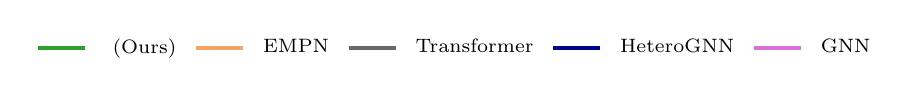
\begin{tikzpicture}
    \tikzstyle{every node}=[font=\scriptsize]
    \definecolor{tabblue}{RGB}{31, 119, 180}
\definecolor{taborange}{RGB}{255, 127, 14}
\definecolor{tabgreen}{RGB}{44, 160, 44}
\definecolor{tabred}{RGB}{214, 39, 40}
\definecolor{tabpurple}{RGB}{148, 103, 189}
\definecolor{tabbrown}{RGB}{140, 86, 75}
\definecolor{tabpink}{RGB}{227, 119, 194}
\definecolor{tabgray}{RGB}{127, 127, 127}
\definecolor{tabolive}{RGB}{188, 189, 34}
\definecolor{tabcyan}{RGB}{23, 190, 207}
\definecolor{lightblue}{RGB}{173, 216, 230}
\definecolor{sandybrown}{RGB}{244, 164, 96}
\definecolor{darkgrey}{RGB}{169, 169, 169}
\definecolor{dimgrey}{RGB}{105, 105, 105}
\definecolor{olivedrab}{RGB}{107, 142, 35}
\definecolor{darkviolet}{RGB}{148, 0, 211}
\definecolor{darkgoldenrod}{RGB}{184, 134, 11}
\definecolor{darkblue}{RGB}{0, 0, 139}
\definecolor{orchid}{RGB}{218, 112, 214}

    \begin{axis}[%
        hide axis,
        xmin=10,
        xmax=50,
        ymin=0,
        ymax=0.1,
        legend style={
            draw=white!15!black,
            legend cell align=left,
            legend columns=5,
            legend style={
                draw=none,
                column sep=1ex,
                line width=1pt,
            }
        },
        ]
        \addlegendimage{line legend, tabgreen, ultra thick} % Thicker line here
        \addlegendentry{\textbf{\model} (Ours)}
        \addlegendimage{line legend, sandybrown, ultra thick} % Thicker line here
        \addlegendentry{EMPN}
        \addlegendimage{line legend, dimgrey, ultra thick} % Thicker line here
        \addlegendentry{Transformer}
        \addlegendimage{line legend, darkblue, ultra thick} % Thicker line here
        \addlegendentry{HeteroGNN}
        \addlegendimage{line legend, orchid, ultra thick} % Thicker line here
        \addlegendentry{GNN}
    \end{axis}
\end{tikzpicture}

    }
    \centering
    \begin{subfigure}[b]{0.32\linewidth}
        \includegraphics[width=\textwidth]{ICLR_2025/Figures/eval_cloth_hanging_equi/eval_full_Isaac-Cloth-Hanging-Multi-v0_eval_all.pdf}
        \caption{Original 3D Space} 
    \end{subfigure}
    \hfill
    \begin{subfigure}[b]{0.32\linewidth}
        \includegraphics[width=\textwidth]{ICLR_2025/Figures/eval_cloth_hanging_equi/eval_half_yaw_Isaac-Cloth-Hanging-Multi-v0_eval_all.pdf}
        \caption{2D Half Circle}
    \end{subfigure}
    \hfill
    \begin{subfigure}[b]{0.32\linewidth}
        \includegraphics[width=\textwidth]{ICLR_2025/Figures/eval_cloth_hanging_equi/eval_quater_yaw_Isaac-Cloth-Hanging-Multi-v0_eval_all.pdf}
        \caption{2D Quarter Circle}
    \end{subfigure}
    \caption{
    \update{
    Performance of different models on the \emph{Cloth-Hanging} task across varying sample spaces. Overall, performance improves as the sample space decreases. In terms of final performance, heterogeneous models outperform homogeneous baselines in most cases, demonstrating the benefits of explicit heterogeneity modeling. Additionally, applying equivariant constraints is critical for achieving superior performance in 3D tasks. More results can be found in Appendix~\ref{appx:further_exp}.
    }
    }
    \vspace{-0.2cm}
    \label{fig:eval_equi}
\end{figure*}
